%%% 实验与评估

\section{实验数据集介绍}

本研究使用的单细胞转录组数据集为 10x Genomics 公司公开发布的经典示例数据集——PBMC 3k 数据集。该数据集包含约 2,700 个外周血单核细胞(Peripheral Blood Mononuclear Cells, PBMC),来自一位健康成年供体。PBMC 包括 T 细胞、B 细胞、自然杀伤细胞和单核细胞等多种免疫相关细胞类型,常作为免疫学研究中的模型系统。

PBMC 3k 数据集采用 10x Genomics Chromium 单细胞 3' RNA 测序平台进行文库构建,并使用 Illumina NextSeq 500 高通量测序仪进行测序。每个细胞平均测序深度约为 69,000 个 reads。原始数据使用 10x Genomics 官方分析工具 Cell Ranger(版本 1.1.0)进行预处理,包括细胞条形码识别、UMI 去重及基因表达矩阵生成。数据结果以稀疏矩阵形式存储,包含每个细胞在各个基因上的表达计数。

本数据集可以在\href{https://cf.10xgenomics.com/samples/cell/pbmc3k/pbmc3k_filtered_gene_bc_matrices.tar.gz}{10XGenomics官网}获取,并可以使用SeuratDisk,scDior等工具转换为h5ad文件。

由于数据来源权威、质量可靠、样本复杂性适中,PBMC 3k 数据集已广泛应用于 Seurat、Scanpy 等单细胞分析工具的功能验证与流程教学中,是验证聚类、降维、批次效应处理等算法性能的标准数据集之一。


\section{实验设计与流程}

本文基于 PBMC 3k 数据集,参考官方流程,实现了单细胞 RNA 测序数据分析的完整流程。以下是使用 Juscan.jl 库进行数据分析的示例:

\subsection{数据读取与质量控制}

Juscan.jl 库使用 Muon.jl 库作为数据存储的基础,支持读取 h5ad 格式的数据文件。数据读取后,使用\code{Juscan.Pp.filter_cells!} 和 \code{Juscan.Pp.filter_genes!} 函数进行细胞和基因的过滤,去除低质量细胞和低表达基因。接着,计算线粒体基因、核糖体基因和血红蛋白基因的表达比例,并根据这些指标进行进一步的质量控制。

\begin{fancybox}{Juscan.jl demo data load and quality control}
\addcontentsline{lot}{table}{代码~\thetcbcounter: Juscan.jl示例:数据读取与质量控制}
\begin{lstlisting}
using Juscan, Muon
using DataFrames, LinearAlgebra, SparseArrays

adata = Juscan.readh5ad("./data/pbmc_3k.h5ad")

############## quality control #################

Juscan.Pp.filter_cells!(adata, min_genes=200)
Juscan.Pp.filter_genes!(adata, min_cells=3)
Juscan.Pp.filter_cells!(adata, max_genes=2300)
Juscan.Pp.filter_cells!(adata, max_counts=10000)

adata.var.mt = startswith.(adata.var_names, "MT-")
adata.var.ribo = startswith.(adata.var_names, "RPS") .| startswith.(adata.var_names, "RPL")
adata.var.hb = occursin.(r"^HB[^P]", adata.var_names)

Juscan.Pp.calculate_qc_metrics!(adata, qc_vars=["mt", "ribo", "hb"])
adata = adata[adata.obs[!, "pct_counts_mt"] .< 8, :]
adata = adata[adata.obs[!, "pct_counts_mt"] .> 0.5, :]

Juscan.Pl.violin(
  adata,
  ["pct_counts_mt", "n_genes_by_counts", "total_counts"];
  width=300,
  height=800,
  fill_alpha=1,
  savefig="/home/lihuax/Pictures/Juscan/qc_violin.png",
)

Juscan.Pl.scatter(
  adata,
  "total_counts",
  "n_genes_by_counts",
  color_key="pct_counts_mt",
  width=800,
  height=800,
  colormap_name="magma",
  savefig="/home/lihuax/Pictures/Juscan/qc_scatter.png",
)

\end{lstlisting}
\end{fancybox}

运行上述代码后,获得处理后的高质量细胞数据集。为了直观展示质量控制的效果,使用小提琴图用于展示线粒体比例、总转录本数量与基因数的分布情况,帮助我们观察数据的整体质量分布;而散点图则揭示了转录本总数与检测到的基因数之间的关系,并以线粒体比例着色,从而更好地识别潜在的异常细胞。

图~\ref{img:Juscan_qc} 所示即为本次质量控制过程中生成的 QC 图像。

\begin{figure}[htbp]
  \centering
  \subfigure{
    \begin{minipage}[b]{.4\linewidth}
       \centering
       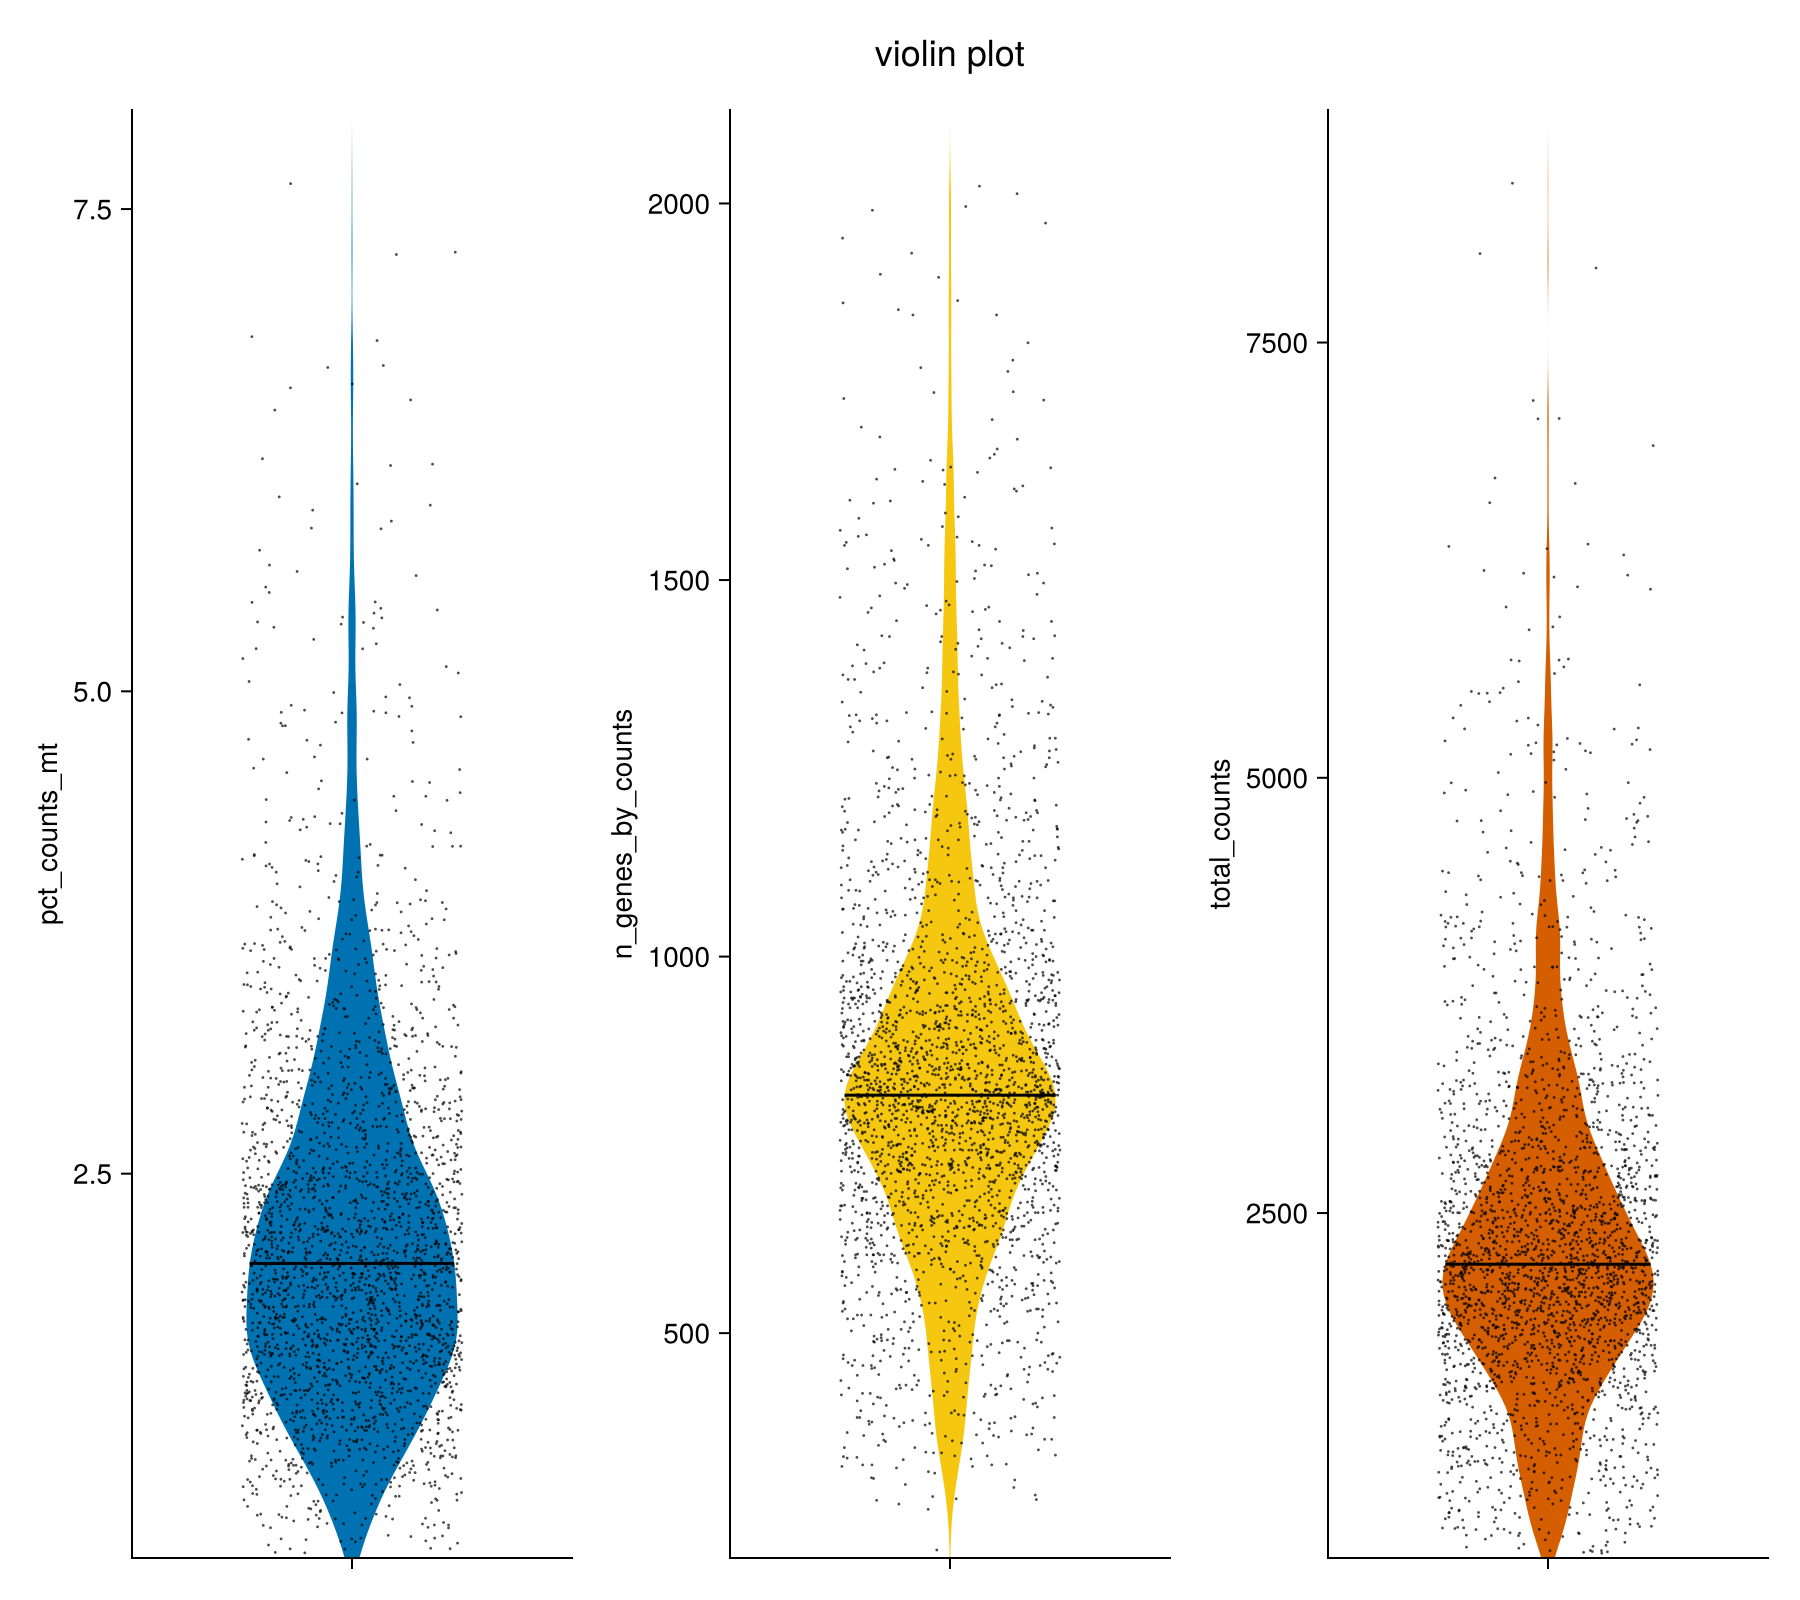
\includegraphics[scale=0.3]{./img/juscan_qc_violin.png}
    \end{minipage}
  }
  \subfigure{
    \begin{minipage}[b]{.4\linewidth}
      \centering
      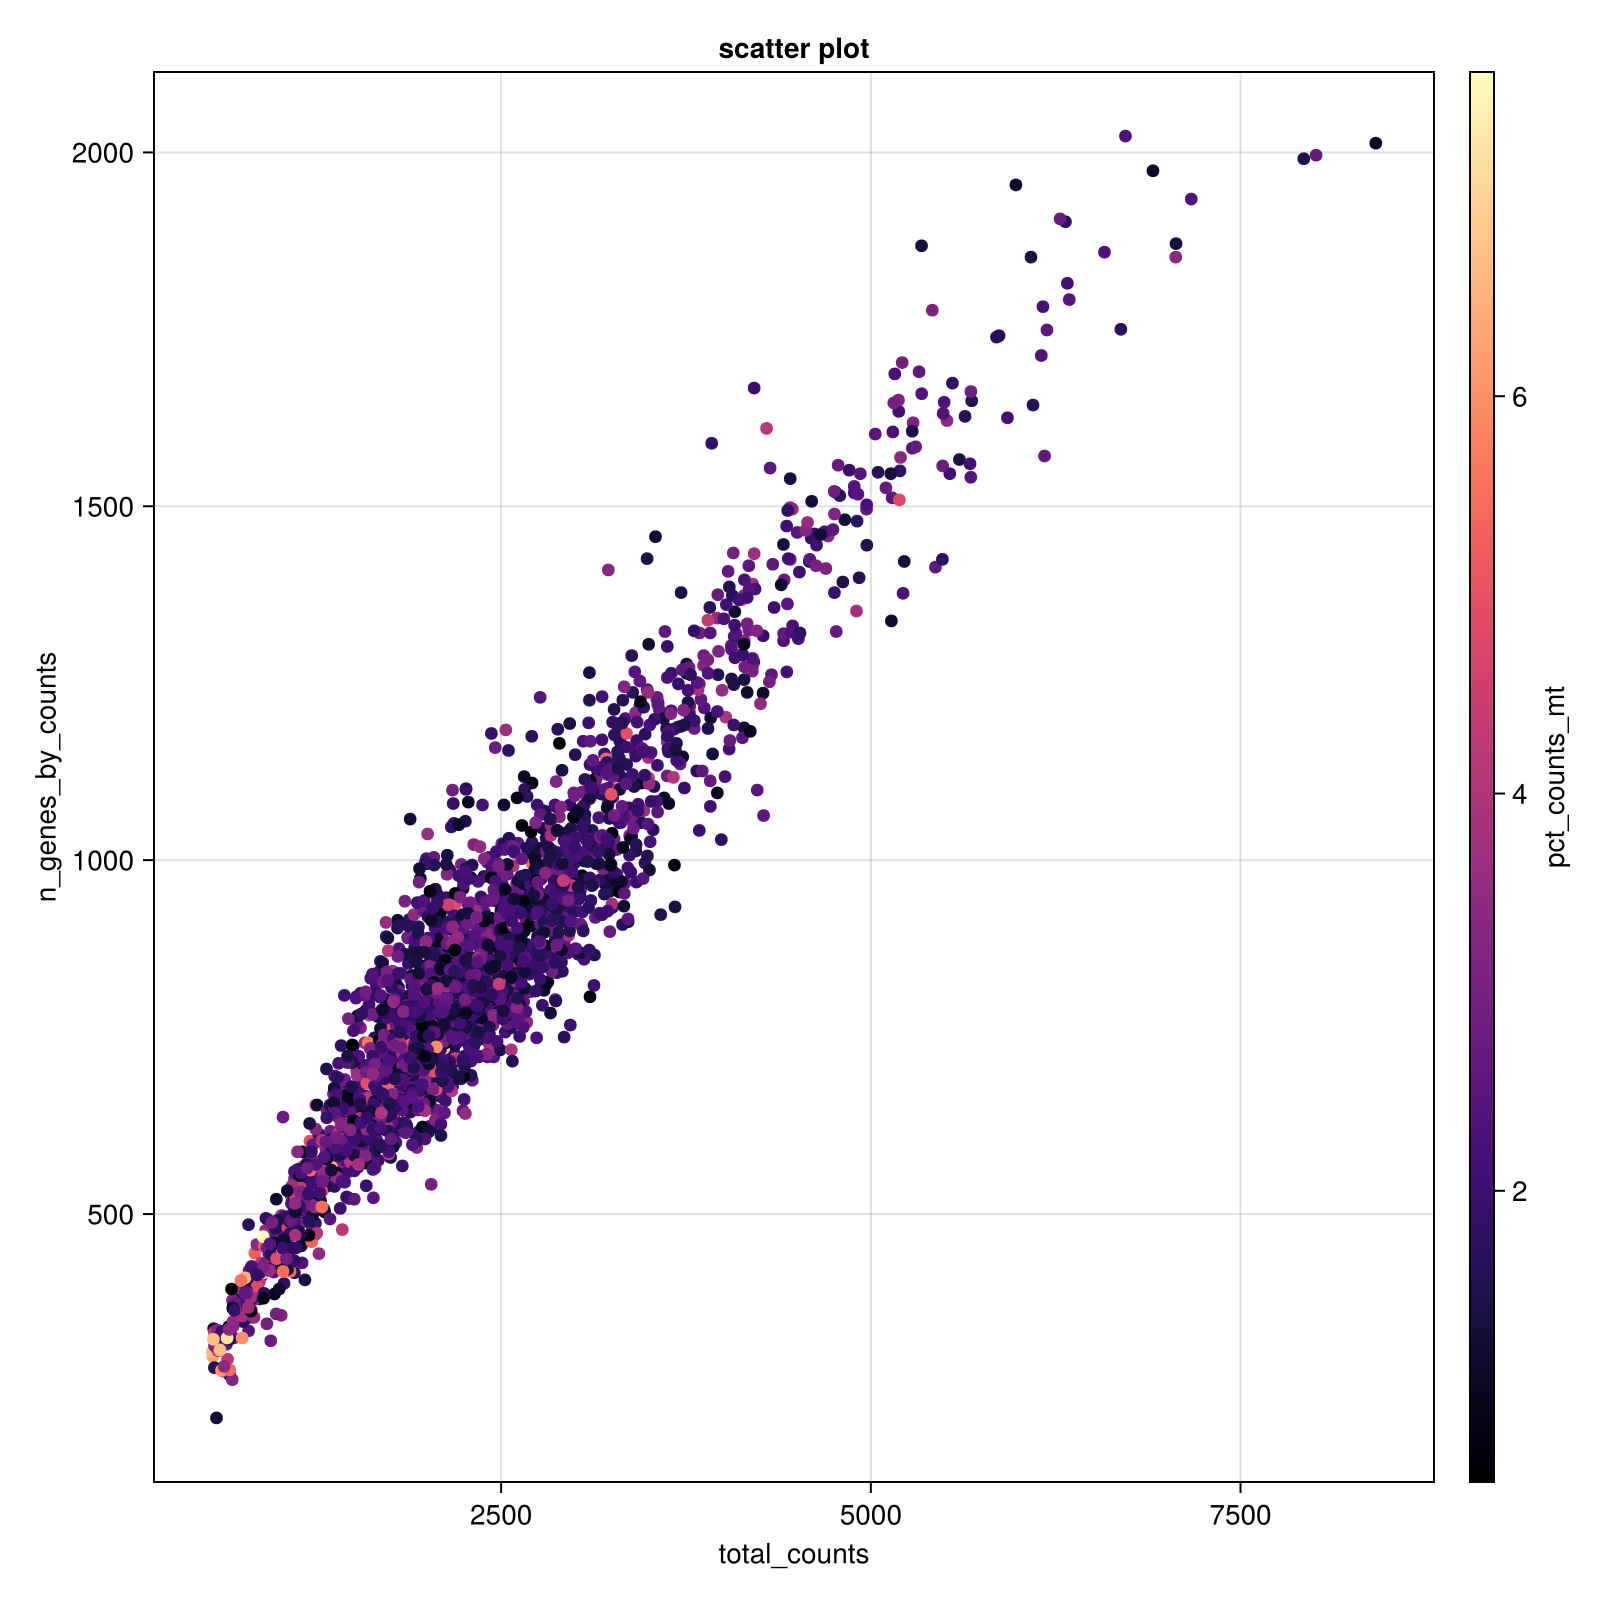
\includegraphics[scale=0.3]{./img/juscan_qc_scatter.png}
    \end{minipage}
  }
  \caption{Juscan.jl质量控制可视化结果}
  \label{img:Juscan_qc}
\end{figure}

\subsection{数据归一化与高变基因}

首先,使用 \code{Juscan.Pp.normalize_total!} 函数对每个细胞的转录本数进行归一化,使其总表达量一致(如 1000),从而消除不同细胞间测序深度的影响。随后,应用 \code{Juscan.Tl.logp1_transform!} 函数对归一化后的数据进行对数变换($log(x+1)log(x+1)$),以缓解表达量跨度过大的问题,使其更符合后续线性模型的假设。

\begin{fancybox}{Juscan.jl normalize and find hvg}
\addcontentsline{lot}{table}{代码~\thetcbcounter: Juscan.jl示例:数据归一化与高变基因}
\begin{lstlisting}
############### normalization #################
adata.layers["normalized"] = deepcopy(adata.X)
Juscan.Pp.normalize_total!(adata, target_sum=1000, layer="normalized")
Juscan.Tl.logp1_transform!(adata, layer="normalized", key_added="normalized_logp1")
adata.layers["normalized_logp1"] = Float64.(adata.layers["normalized_logp1"])

############### highly variable genes #################
Juscan.Tl.highly_variable_genes!(adata, n_top_genes=2000, layer="normalized_logp1")
Juscan.Pl.hvg_scatter(adata, savefig="/home/lihuax/Pictures/Juscan/hvg_scatter.png")
\end{lstlisting}
\end{fancybox}

在归一化的基础上,使用 \code{Juscan.Tl.highly_variable_genes!} 方法从全基因集中筛选出表达波动性最强的 2000 个基因。这些基因包含了最丰富的生物学信号,是降维与聚类分析的核心输入。

图~\ref{img:hvg} 展示了PCA肘部图和高变基因的分布图,肘部图用于后续分析中选择pca维度数字而hvg图中显示了高变基因的分布,其中深色点为筛选出的高变基因。

\begin{figure}[htbp]
  \centering
  \subfigure{
    \begin{minipage}[b]{.27\linewidth}
       \centering
       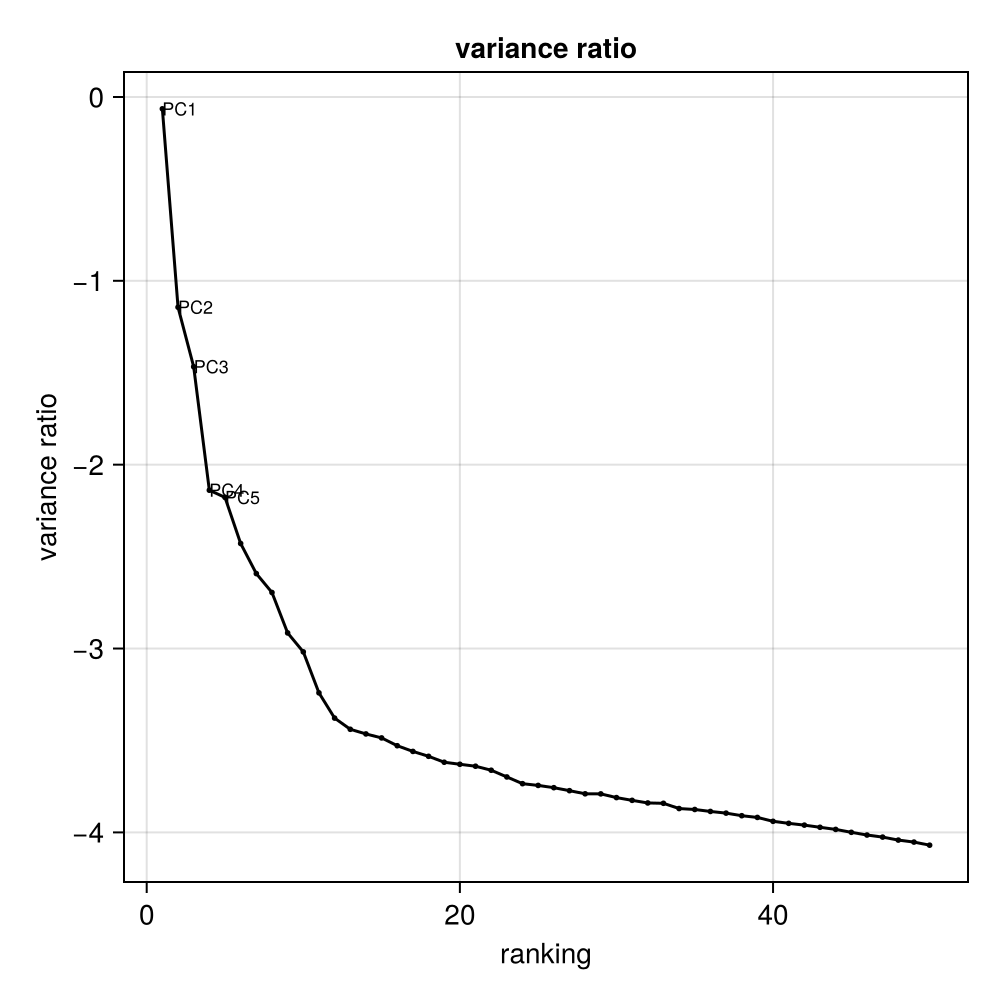
\includegraphics[width=\textwidth]{./img/juscan_variance_ratio.png}
    \end{minipage}
  }
  \subfigure{
    \begin{minipage}[b]{.7\linewidth}
      \centering
      % 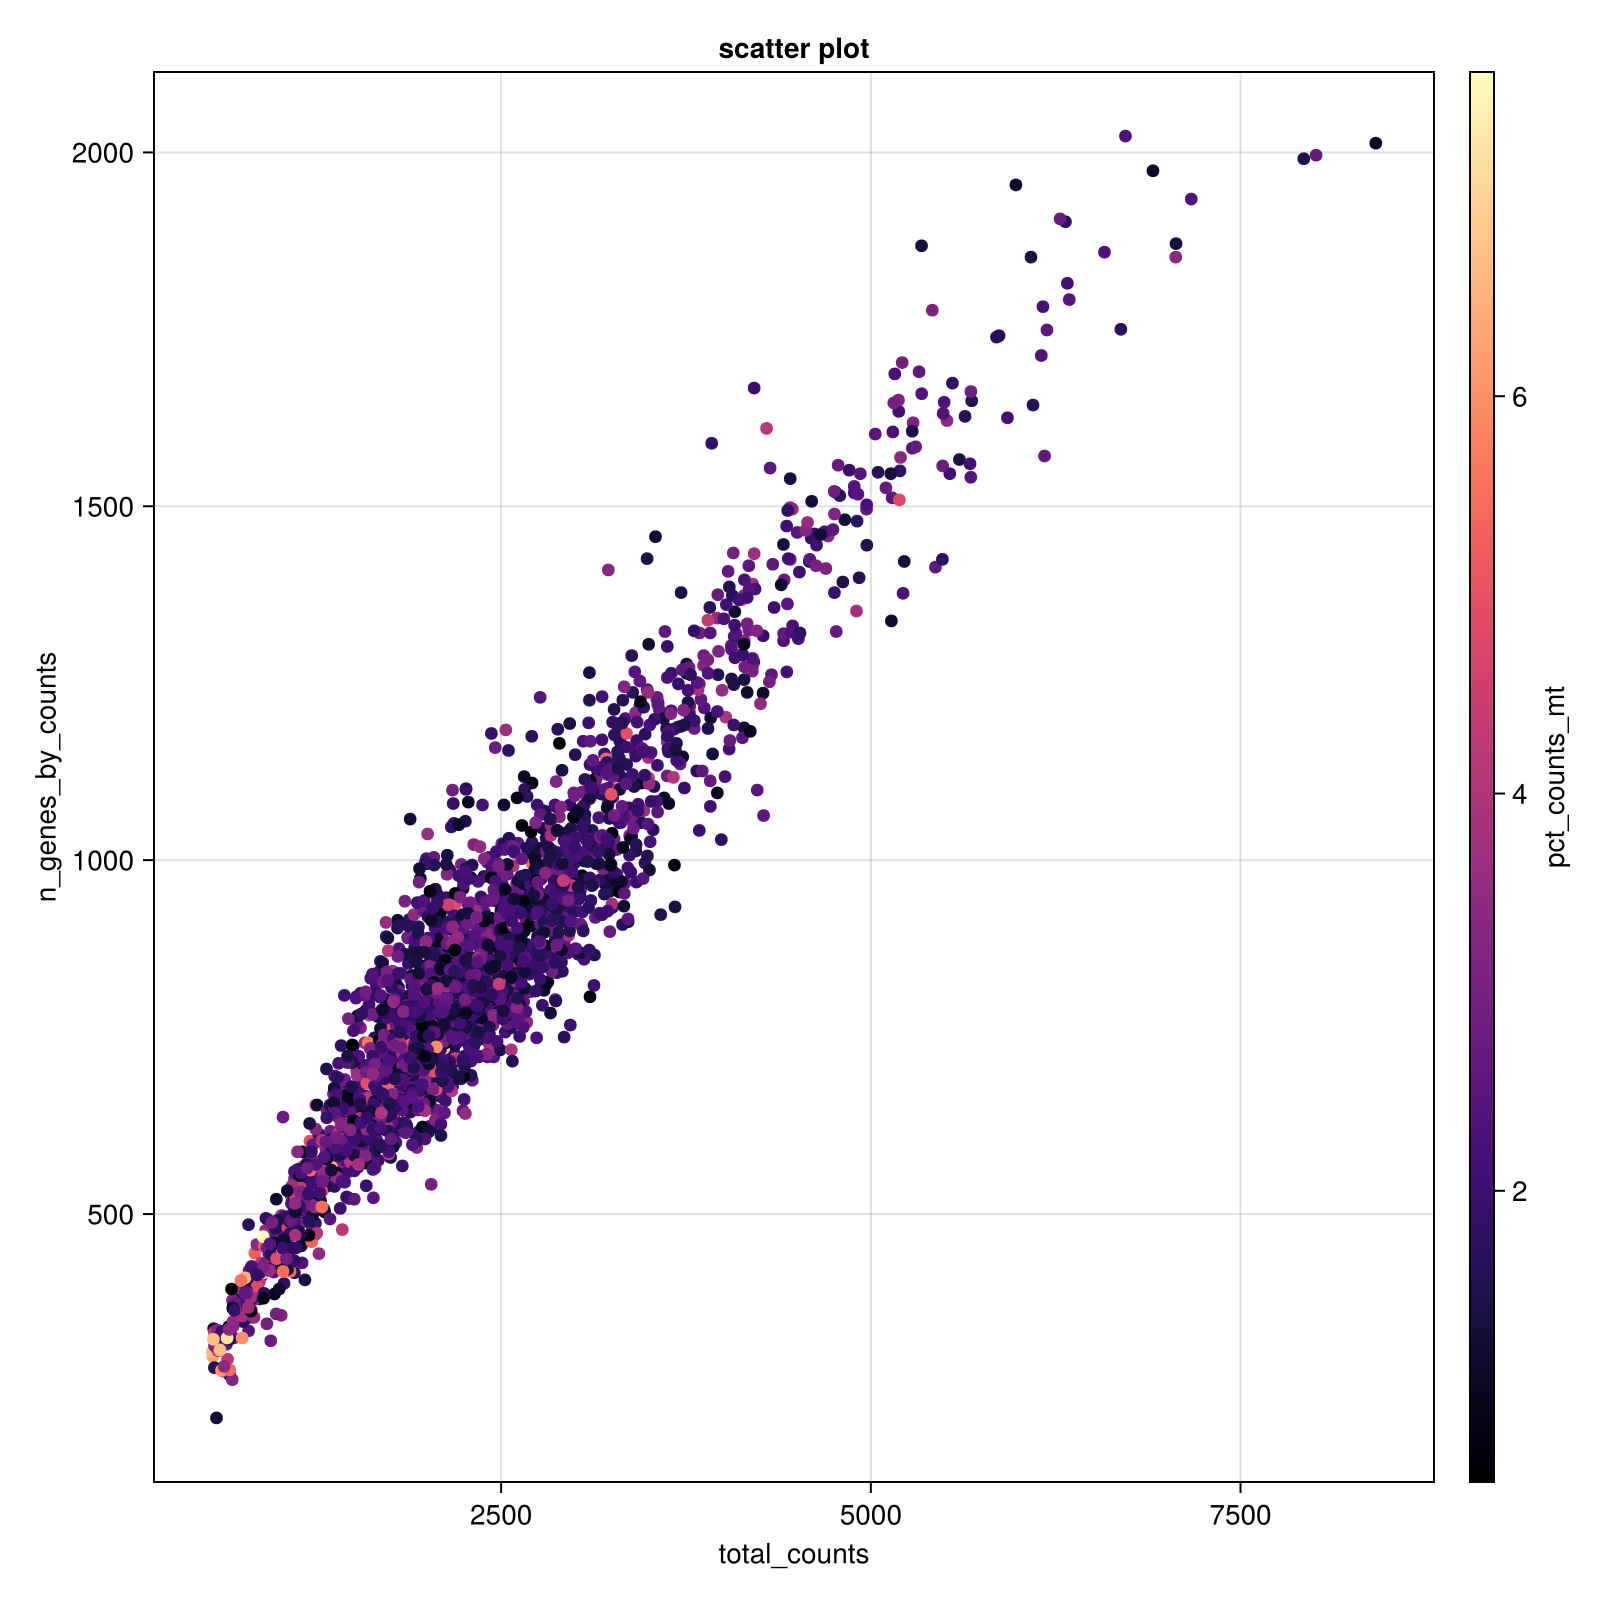
\includegraphics[scale=0.4]{./img/juscan_qc_scatter.png}
        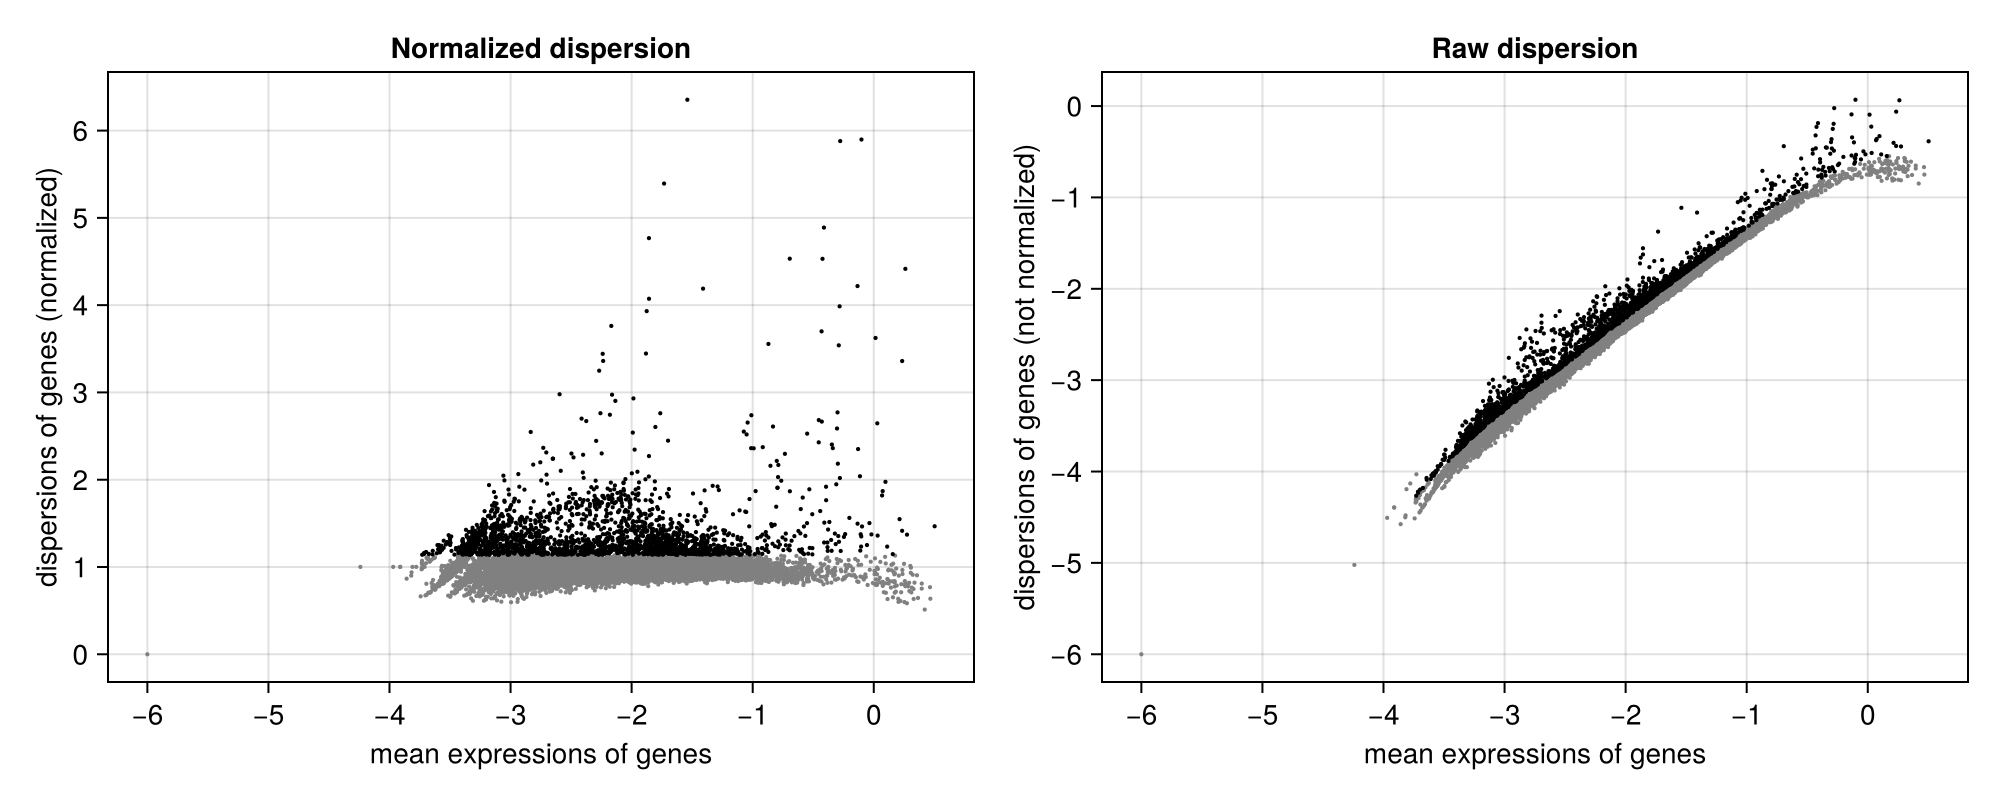
\includegraphics[width=\textwidth]{img/juscan_hvg_scatter.png}
    \end{minipage}
  }
  \caption{Juscan.jl归一化和高变基因可视化结果}
  \label{img:hvg}
\end{figure}

\subsection{降维与聚类}

在完成归一化与高变基因筛选之后,进行高维数据的压缩与结构发现。首先,通过 \code{Juscan.Tl.subset_to_hvg!} 筛选前 1000 个高变基因,以提取最具代表性的表达信号。随后,我们使用 \code{Juscan.Tl.pca!} 执行主成分分析(PCA),将原始维度浓缩为若干主成分,同时保存方差贡献比,便于选择合适的维度数进行后续分析。

紧接着,我们通过社区发现算法对 PCA 空间中的细胞进行聚类,以发现细胞的潜在亚群结构。通过 \code{Juscan.Tl.umap!} 函数进一步将 PCA 结果降维至二维空间,用于可视化聚类结果。

\begin{fancybox}{Juscan.jl dimensionality reduction and clustering}
\addcontentsline{lot}{table}{代码~\thetcbcounter: Juscan.jl示例:数据降维与聚类}
\begin{lstlisting}
############### dimensionality reduction #################
Juscan.Tl.subset_to_hvg!(adata; layer="normalized_logp2", n_top_genes=1000)

Juscan.Tl.pca!(adata; layer="normalized_logp1", key_added="pca", n_pcs=50)
Juscan.Pl.plot_variance_ratio(adata, savefig="/home/lihuax/Pictures/Juscan/variance_ratio.png")

############### clustering #################
Juscan.Tl.clustering!(adata, reduction="pca", use_pca=10, resolution=0.6)
Juscan.Tl.umap!(
  adata;
  key_added="umap",
  use_pca="pca",
  n_pcs=10,
  min_dist=0.5,
  n_neighbors=30,
)
Juscan.Pl.plot_umap(
  adata,
  color_by="clusters_latest",
  key="umap",
  savefig="/home/lihuax/Pictures/Juscan/clusters.png",
)
\end{lstlisting}
\end{fancybox}

图~\ref{img:clusters umap plot} 展示了 UMAP 嵌入空间中的聚类结果。每个点代表一个细胞,颜色区分不同的聚类标签。聚类结果的清晰分离,提示着数据中存在明显的生物学异质性,可能对应于不同类型的免疫细胞或功能状态。通过这样的降维可视化图,我们不仅能够观察整体结构,还能识别边缘群体与潜在的亚群细胞,为后续的注释与生物学解释奠定坚实基础。

\begin{figure}[htbp]
  \centering
  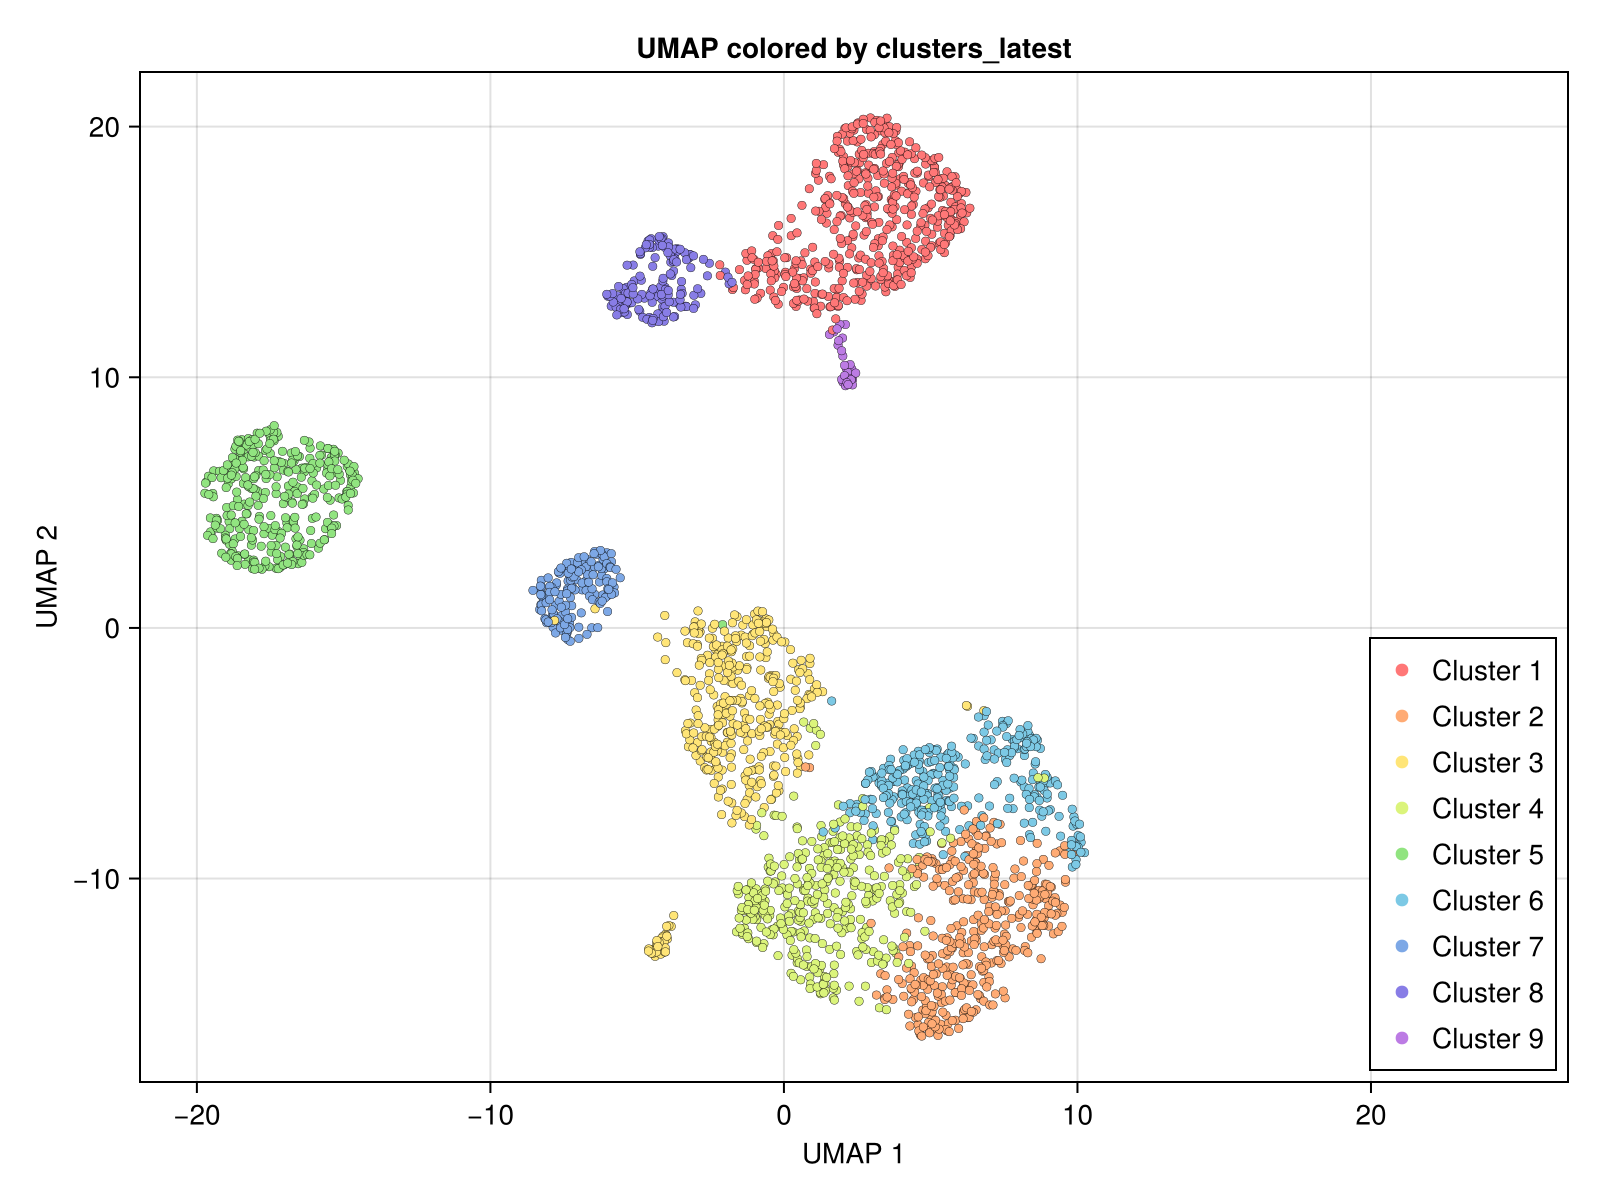
\includegraphics[width=0.7\textwidth]{img/juscan_clusters.png}
  \caption{Juscan.jl聚类结果umap可视化}
  \label{img:clusters umap plot}
\end{figure}

\section{性能评估}

为了全面评估不同语言实现对单细胞 RNA 测序数据处理流程的效率与性能差异,本文基于 PBMC 3k 数据集,分别使用 Julia、Python 与 R 三种主流语言构建了统一流程的 benchmark 测试系统。三种实现版本在逻辑结构、分析步骤及参数设置上保持一致,涵盖典型的单细胞分析流程,包括质量控制、归一化处理、高变基因选择、主成分分析(PCA)、聚类分析与 UMAP 可视化。

其中,Julia 的测试基于\code{BenchmarkTools.jl} 库, python和R分别使用\code{time}模块和\code{system.time}方法自行构建性能测试函数。
在每个步骤中,实验统一采用 100 次重复采样方式对每个函数进行性能测量,并最终输出时间与内存占用的统计汇总结果(CSV 格式)。

详细的测试代码请见附件。

\subsection{Seurat对比juscan.jl评估结果}

如下图\ref{img:r_vs_julia}是对比 Seurat 和 juscan.jl 的性能评估结果。

由于Seurat和Juscan的逻辑差异比较大,fiter和计算质量控制矩阵步骤没有被单独封装为函数,因此这里并没比较这些步骤的效率。

而对于已经比较的步骤,Juscan的效率明显优于Seurat,尤其在归一化,降维和聚类方面,Juscan的性能优势更为明显。

\begin{figure}[htbp]
  \centering
  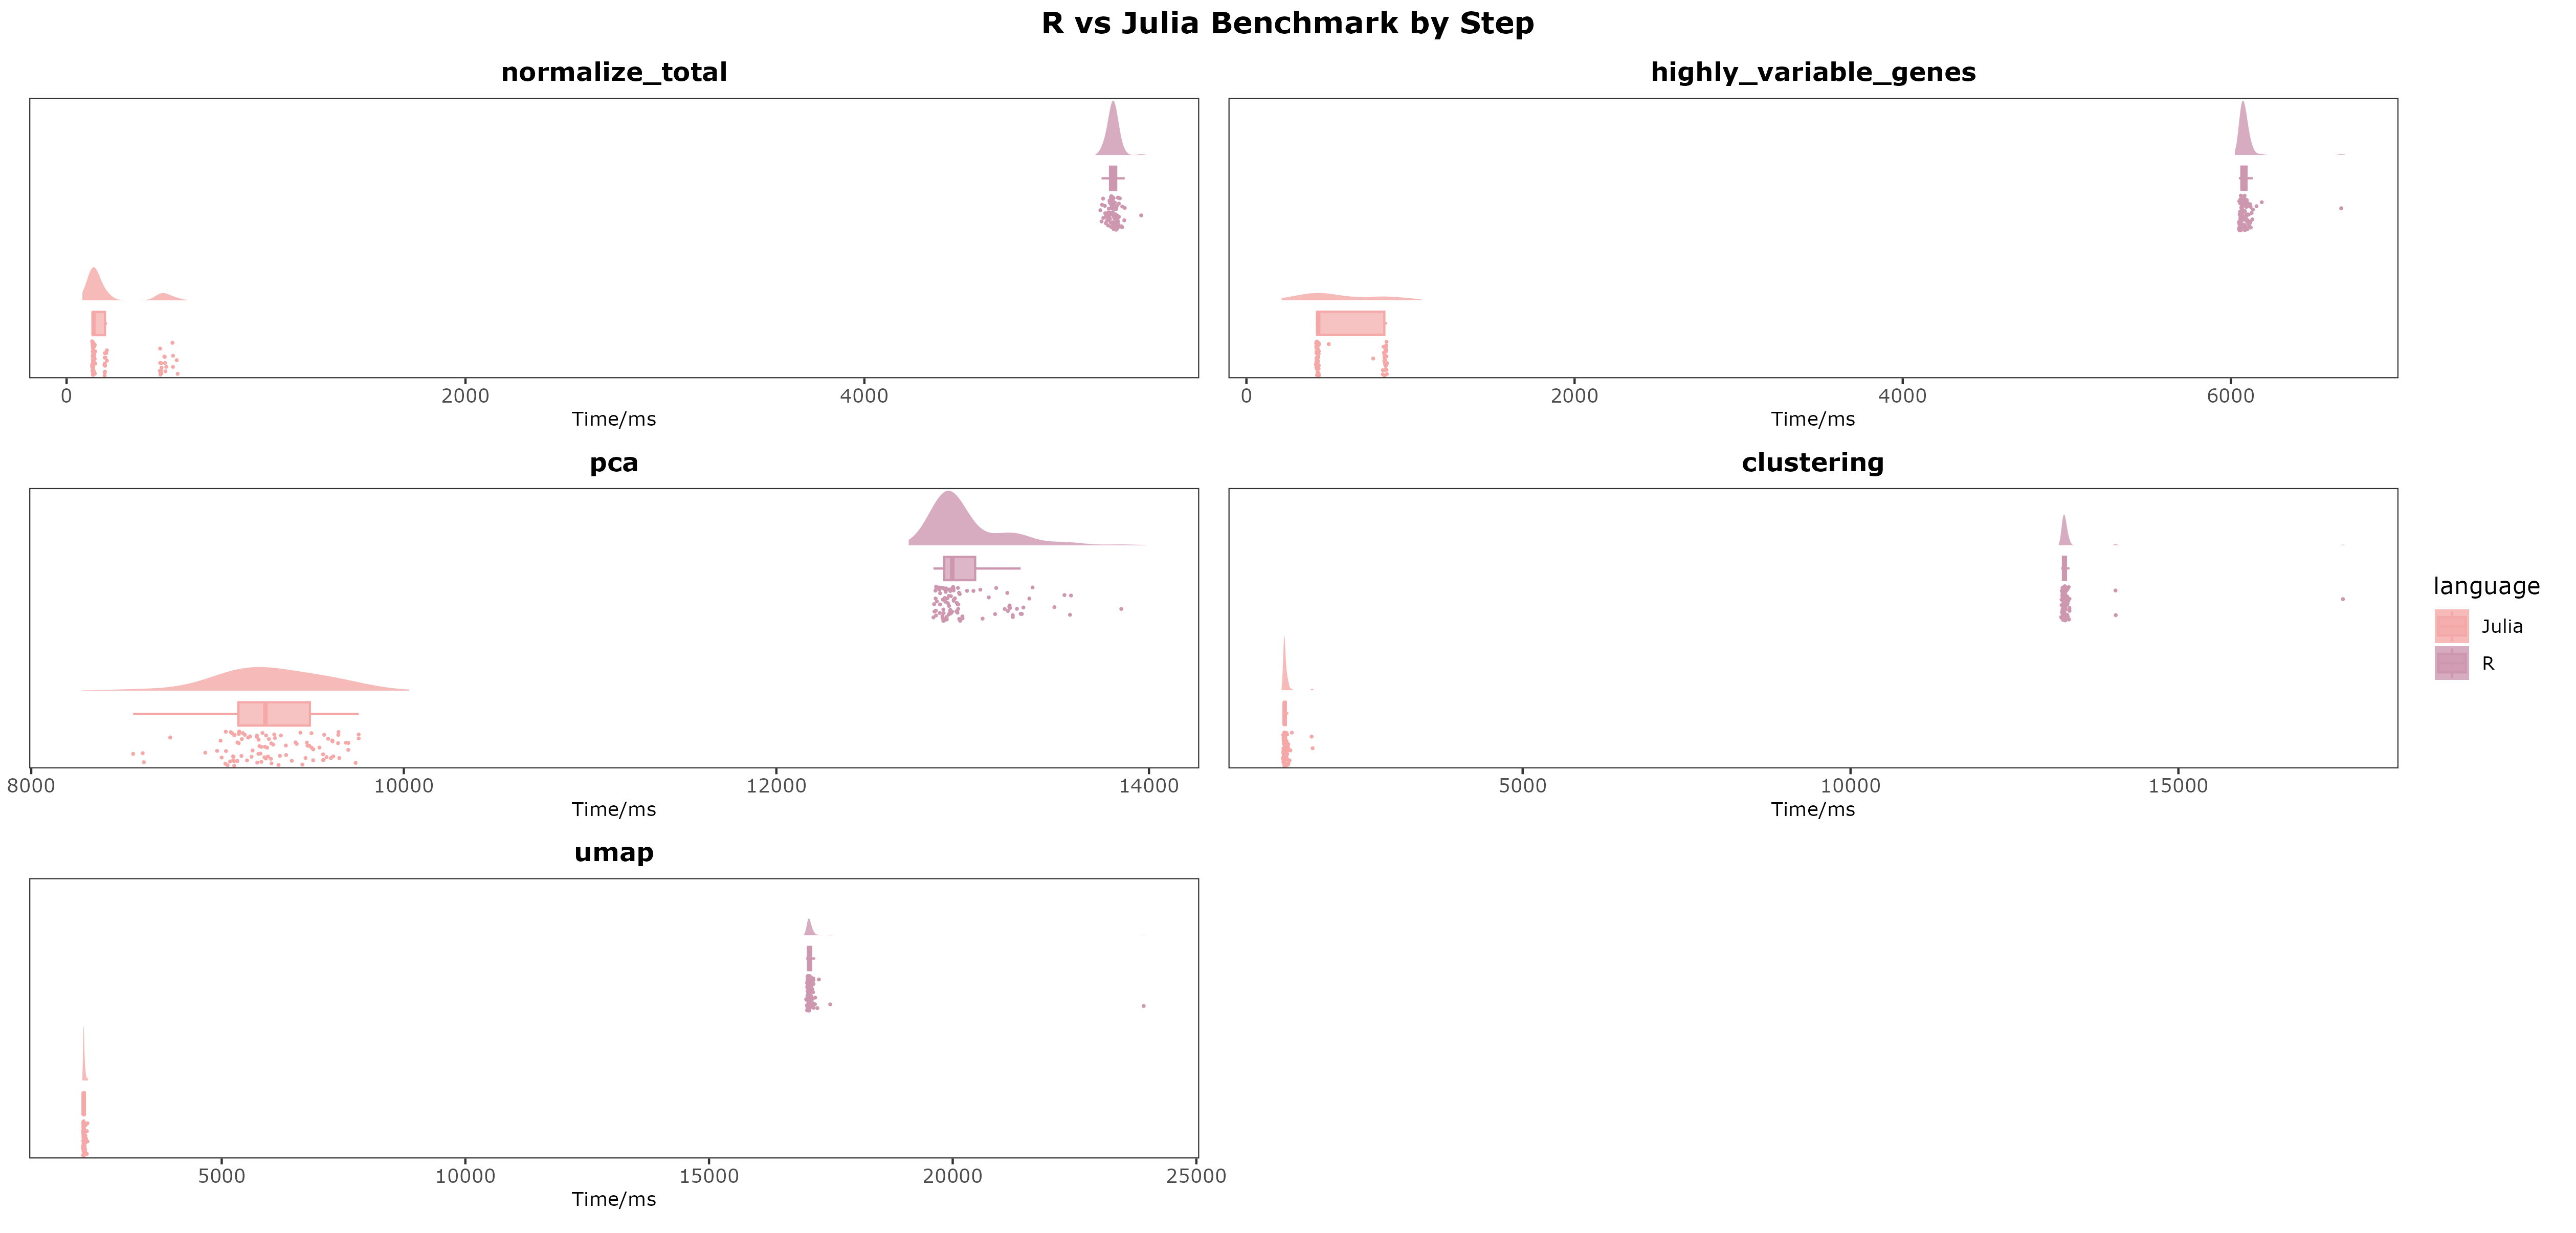
\includegraphics[width=0.7\textwidth]{img/r_vs_julia.png}
  \caption{Juscan.jl与Seurat性能对比}
  \label{img:r_vs_julia}
\end{figure}

\subsection{scanpy对比juscan.jl评估结果}

如下图\ref{img:python_vs_julia}是对比 scanpy 和 juscan.jl 的性能评估结果。

可以明显看到,python在数据读取、归一化、PCA 和 UMAP 等步骤上均表现出显著的性能优势,尤其在降维方面。
另外Juscan的性能表现并不稳定,在不同的测试中,性能波动较大,可能与 Julia 的 JIT 编译机制有关。

总之,在归一化和降维,聚类等步骤上,Python 的性能明显优于 Julia,Juscan.jl任有恒大的进步空间。

\begin{figure}[htbp]
  \centering
  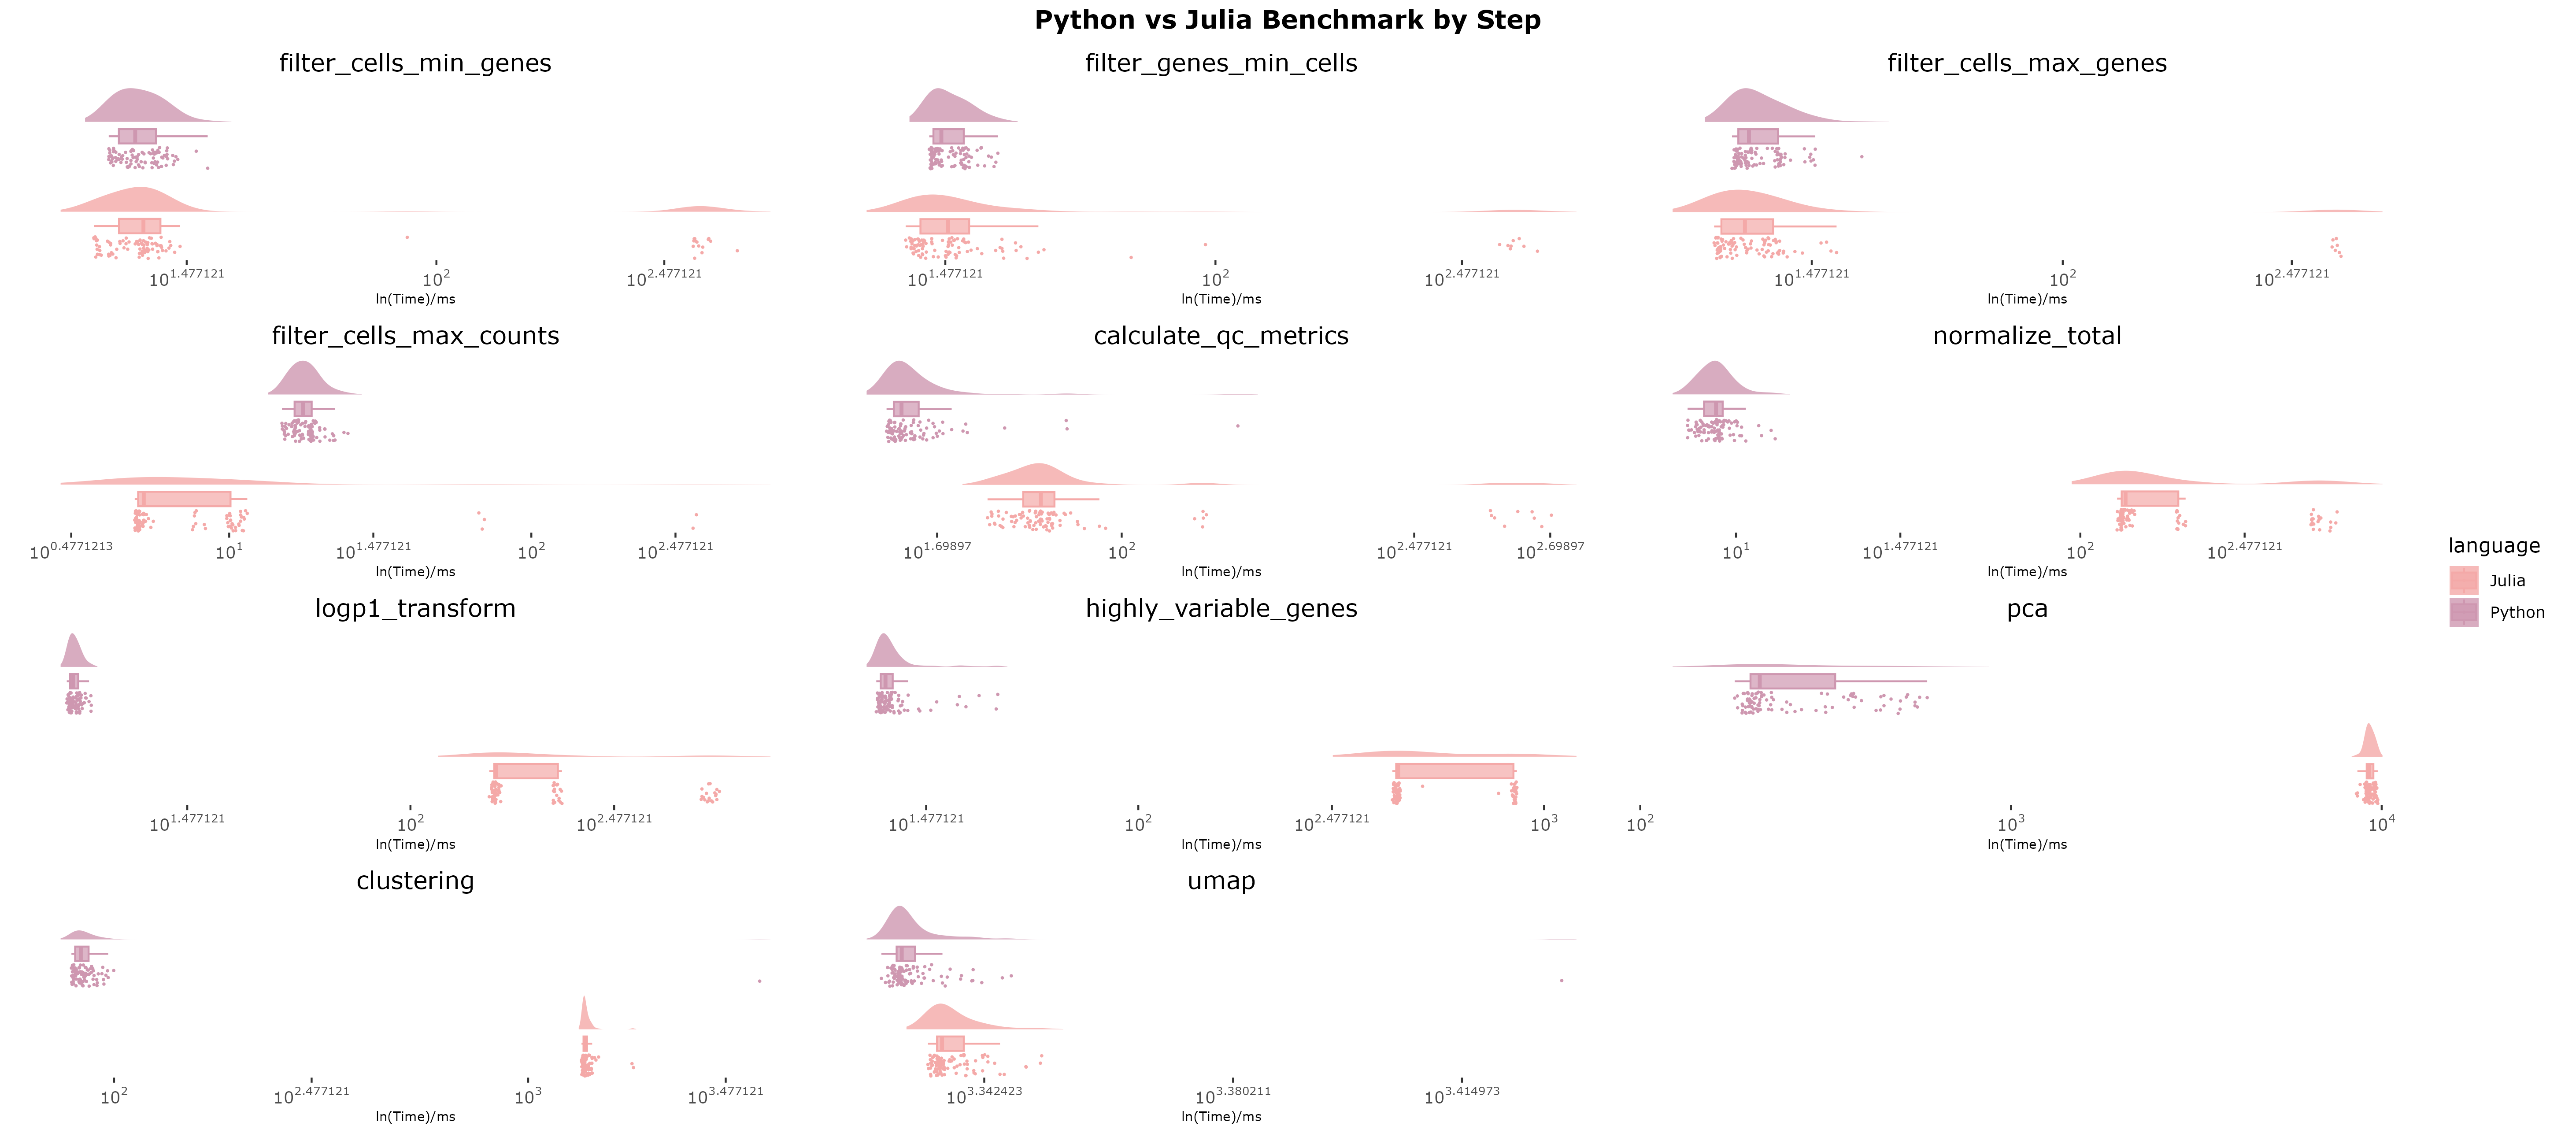
\includegraphics[width=0.8\textwidth]{img/python_vs_julia.png}
  \caption{Juscan.jl与Scanpy性能对比}
  \label{img:python_vs_julia}
\end{figure}

